\section{Qu’est-ce qu’un graph}
Un graphe est un modèle abstrait de dessins de réseaux reliant des objets [11]. Ces modèles sont constitués par la donnée de sommets (aussi appelés nœuds), et d'arêtes (aussi appelées liens ou relation) entre ces sommets ; ces arêtes sont parfois non-symétriques (les graphes sont alors dits orientés) et sont appelés des flèches.\\

\begin{figure}[h!]  
  \centering
    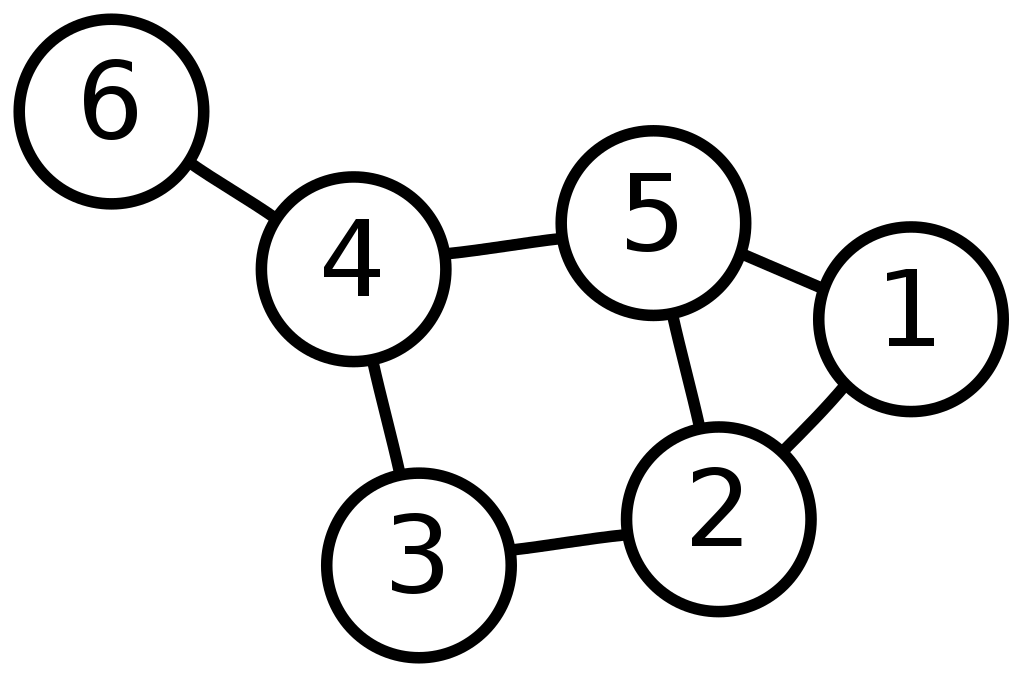
\includegraphics[width=0.5 \textwidth]{chapitre2/Figures/GraphNonOriontee.png}
  \caption{Graphe non orientée}
  \centering
    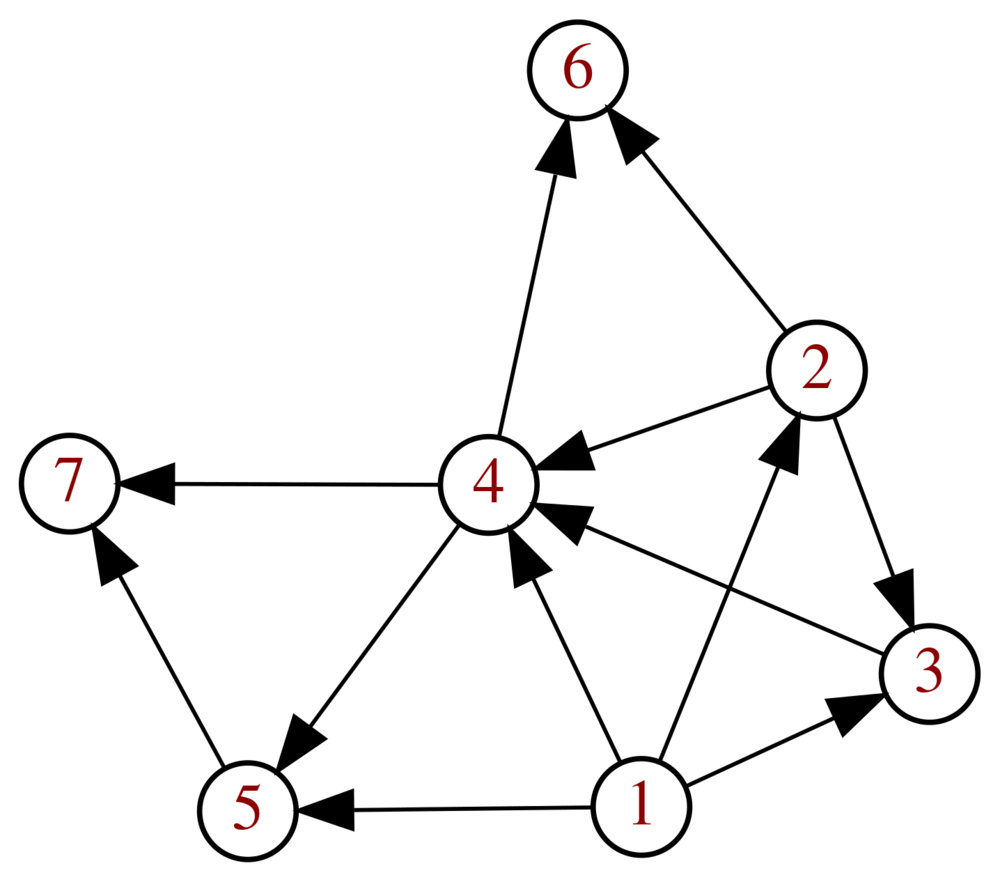
\includegraphics[width=0.5 \textwidth]{chapitre2/Figures/GraphOriontee.png}
  \caption{Graphe orientée}
\end{figure}

On ne peut pas parler des graphes dans le contexte académique sans parler de la théorie des graphes, c’est la discipline mathématique et informatique qui étudie les graphes. La théorie des graphes il a comme origine le mathématicien suisse Leonhard Euler, qui en 1735 a présenté à l'Académie de Saint-Pétersbourg un article qui traitait le problème des sept ponts de Königsberg. Le problème consistait à traverser une ville appelée Königsberg, cette ville est construite autour de deux îles situées sur un fleuve et reliées entre elles par un pont. Six autres ponts relient les rives de la rivière à l'une ou l'autre des deux îles, comme représentés dans la figure ci dessus. Le problème consiste à déterminer s'il existe ou non une promenade dans les rues de Königsberg permettant, à partir d'un point de départ au choix, de passer une et une seule fois par chaque pont, et de revenir à son point de départ, étant entendu qu'on ne peut traverser la rivière qu'en passant sur les ponts.\\

\begin{figure}[h!]  
  \centering
    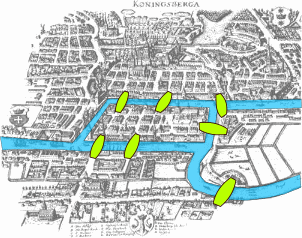
\includegraphics[width=0.4 \textwidth]{chapitre2/Figures/Konigsberg_bridges.png}
  \caption{Ville de Königsberg et ces sept ponts}
  \centering
    \includegraphics[width=0.4 \textwidth]{chapitre2/Figures/Königsberg_graph.svg.png}
  \caption{Modéle en graphe orionté de la ville de Königsberg}
\end{figure}

Les algorithmes élaborés pour résoudre des problèmes concernant les objets de cette théorie ont de nombreuses applications dans tous les domaines liés à la notion de réseau (réseau social, réseau informatique, télécommunications, etc.) et dans bien d'autres domaines.\\



\textbf{Terminal de paiement électronique :} Le terminal de paiement électronique (TPE) est un système matériel pour le traitement des paiements par carte dans les magasins. 

%


\textbf{ProwerCard (PWC) :} PowerCARD est la suite complète de solutions de HPS qui couvre toute la chaîne de valeur des paiements en permettant des paiements innovants grâce à sa solution omni-channel qui permet le traitement de toutes les transactions en provenance de tous les canaux initiées par n'importe quel moyen de paiement.

\textbf{PowerCARD-xPOS :} La solution PowerCARD-xPOS et l'une de la suite complète de solutions de HPS. PowerCARD-xPOS peut aider les fournisseurs de paiements, les détaillants et les banques à piloter les appareils, changer d'autorisation, capturer les données de transaction et gérer la compensation et le règlement de manière rentable, dynamique et efficace, et à déployer rapidement de nouveaux services et simplement un déploiement global des appareils, tout en réduisant au minimum les coûts de maintenance et d'administration.

\textbf{Pos monitoring :} le Pos monitoring est une partie de la solution PowerCARD-xPOS qui peut aider les utilisateurs des TPE à la supervision de leurs TPE.